


In this chapter I study the three methods for approximating the Langevin likelihood presented in chapter~\ref{chap: methods} by using simulations of the Langevin process. Throughout this chapter I will be simulating from the Langevin using the Euler-Maruyama method with the perlin noise Covariates presented in figure~\ref{fig:covariate plots} and a time resolution of $\Delta_t =0.01$.




\section{Extended Kalman Filter}
\label{sec: EKF test}
To test the likelihood approximation using the Extended Kalman filter, 100 tracks were simulated each with 5000 observations with a resolution of $\Delta t = 0.1$. For each track, the parameters $\gamma^2$ and $\bm \beta$ were estimated using both the EKF likelihood and the estimator described in section~\ref{sec: estimating parameters}. The number of steps used in the extended Kalman filter was 10. From these estimates box-plots were made comparing the two methods for each of the parameters. The code used to implement this experiment can be found in the git hub repository in appendix~\ref{Appendix: github repo}. the results are shown in figure~\ref{fig:EKF_thin_boxplot}.

 

\begin{figure}[H]
    \centering
    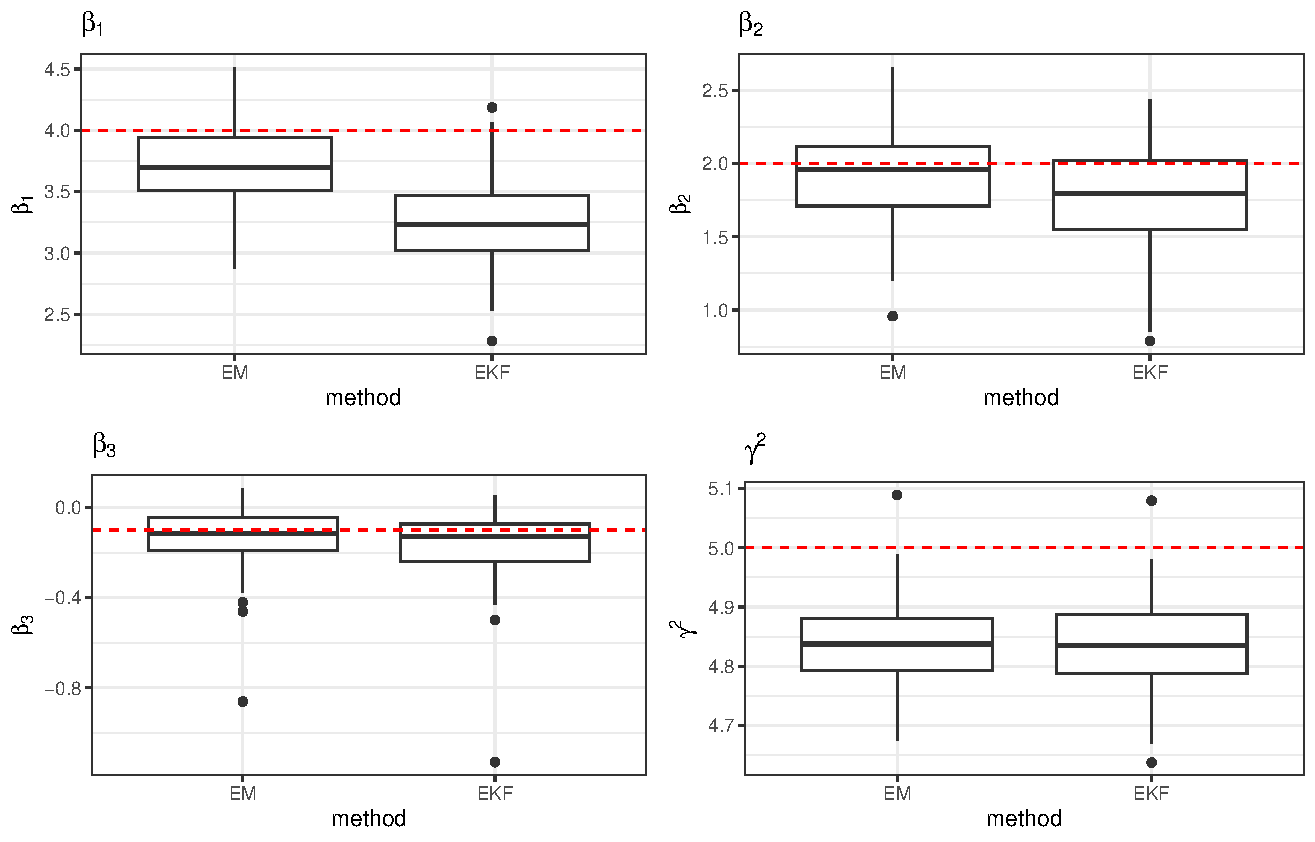
\includegraphics[width=\linewidth]{Images/Results/EM EKF plot.pdf}
    \caption[Euler-Maruyama and extended Kalman filter estimates]{Boxplots of estimated parameters for tracks with 5000 observation using the Euler-Maruyama method to the left and the extended Kalman filter to the right. The red line indicates the true value of the parameter.}
    \label{fig:EKF_thin_boxplot}
\end{figure}

Figure~\ref{fig:EM_thin_boxplot} shows that there is little or no improvement in the estimates from using the extended Kalman filter. for the $\bm \beta$ parameters, then mean estimated parameter is further from the true value of the parameter than the mean of the estimates using the Euler-Maruyama method. For the estimates of $\gamma^2$ however, the mean of the estimates using the extended Kalman filter is slightly closer to the true value of the parameter than the mean of the estimates using the Euler Maruyama method. Overall there is an observable bias in the estimates using both these methods in all of the parameters.

\section{Brownian Bridge Importance Sampling Likelihood}
\label{sec: BB test}
To find estimates using the Brownian bridge importance sampling likelihoods, The method "L-BFGS-B" was used in the function "optim" from the R package "optim". In addition a gradient was specified, a derivation for which can be found in appendix\ref{Appendix C}. 


Both of the Brownian bridge importance sampling methods were tested in three different scenarios. In the first scenario, the methods were used to find estimates of tracks with 5000 observation and three types of thinning $\Delta_t =\{0.1, 0.5, 1\}$. In the second scenario 100 tracks were simulated and the parameters $\bm \beta$ and $\gamma^2$ were estimated using the two methods with three values of number of bridge nodes $N=\{4, 9, 49, 99\}$. In the third scenario 100 tracks were simulated, then the parameters $\bm \beta$ and $\gamma^2$ were estimated using the two methods with 5 values of numbers of bridges $M=\{5,10,50,100,200\}$. 


\subsection{Scenario 1}
To study the effect of the time difference between observations, $\Delta_t$, on the Brownian bridge importance sampling likelihood estimates, 100 tracks were simulated from the Langevin process. These tracks were thinned, so that the interval between observation were $\Delta_t \in \{0.1, \ 0.5, \ 1\}$. They were then shortened so each track contained 5000 observations. For each of these 300 tracks, the parameters $\gamma^2$ and $\bm \beta$ were estimated using the maximum of the brownian bridge importance sampling likelihood. The number of bridges used was $M=50$ and the number of nodes was $N =\{9,49,99\}$ for the respective values of $\Delta_t$. The result of these estimations using the Brownian bridge importance sampling likelihood are shown in figure~\ref{fig:varying dt boxplot BB}, and the result using precomputed Brownian bridges are shown in figure~\ref{fig:varying dt boxplot precomputed BB}

\begin{figure}[H]
    \centering
    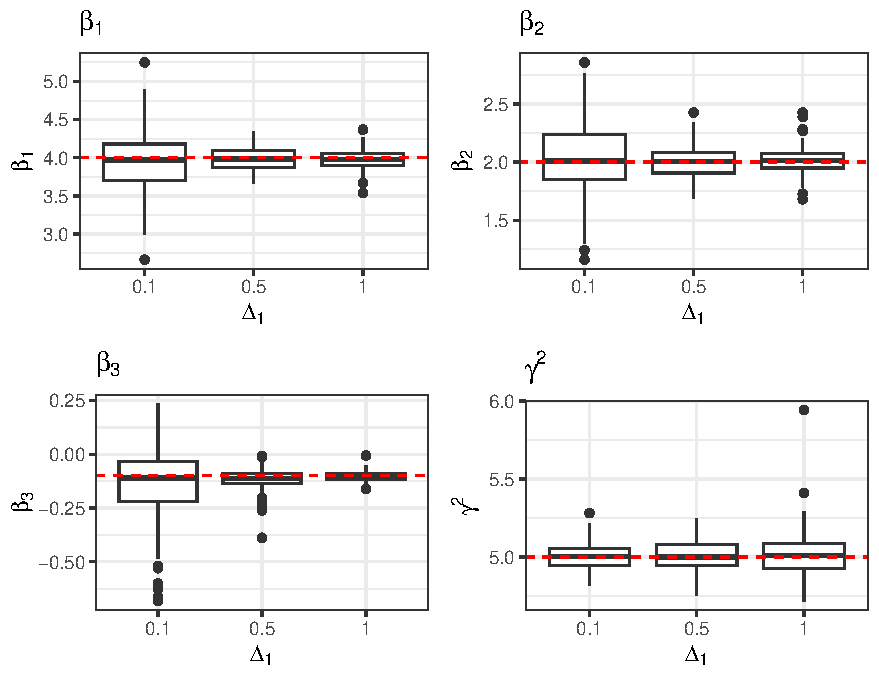
\includegraphics[width=\linewidth]{Images/Results/varying dt plot brownian bridge likelihood.pdf}
    \caption[Box plots of Parameter Estimates using Brownian bridge importance sampling at different sampling intervals]{box plots showing how the parameter estimates using the importance sampling estimator is affected by the time interval between observations. The red dotted lines show the true values of the parameters.}
    \label{fig:varying dt boxplot BB}
\end{figure}

There is no observable bias any of the parameter estimates in figure~\ref{fig:varying dt boxplot BB}. This is in contrast to what is observed in the EM-estimates in figure~\ref{fig:EM_thin_boxplot}, where there is an increasing bias as the time difference between observations increases. For $\gamma^2$, when we have $\Delta_t=1$, there are two outliers among the estimates that have overestimated the parameter to a large extent. 

The same pattern as was observed in figure~\ref{fig:EM_thin_boxplot}, where the variance of the parameter estimates of $\bm \beta$ is reduced as $\Delta_t$ increases, is also observed in figure~\ref{fig:varying dt boxplot BB}. For $\gamma^2$ there is a slight increase in the variance of the estimates as $\Delta_t$ increases, which is also the same as what was observed in figure~\ref{fig:EM_thin_boxplot}.



\begin{figure}[H]
    \centering
    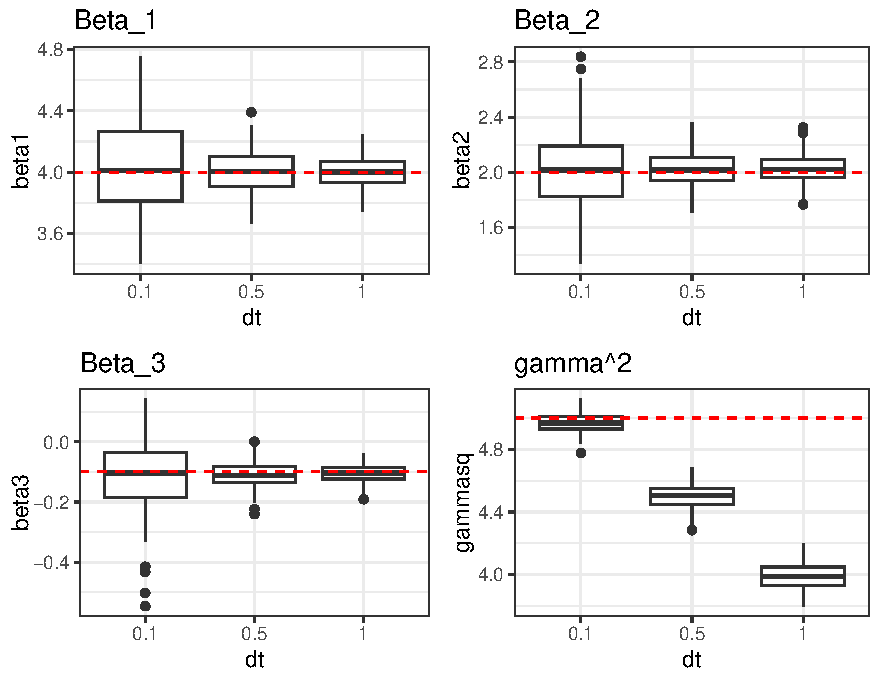
\includegraphics[width=\linewidth]{Images/Results/varying dt estimates precomputed BB.pdf}
    \caption[Box plots of Parameter Estimates using pre-computed Brownian bridge importance sampling at different sampling intervals]{box plots showing how the parameter estimates using the importance sampling estimator, with pre-computed Brownian bridges is affected by the time interval between observations. The red dotted lines show the true values of the parameters.}
    \label{fig:varying dt boxplot precomputed BB}
\end{figure}


From figure~\ref{fig:varying dt boxplot precomputed BB} we can see that the estimates from the simulated tracks using the precomputed Brownian bridge importance sampling likelihood showed no bias in any of the $\bm \beta$-parameters, which is in contrast to the results using the Euler-Maruyama method where there were bias in the estimates for all the values of $\Delta_t$ used in figure~\ref{fig:varying dt boxplot precomputed BB}. An observation that is consistent with that of the Euler-Maruyama estimates is that the variance of the $\bm \beta$-estimates is reduced as the time difference between observation $\Delta_t$ increases. 

\

In addition there is a bias in the $\gamma^2$-estimates, which is also something seen in the Euler-Maruyama estimates. The estimates using precomputed Brownian bridge importance sampling likelihood, do however have a smaller bias than is observed for the Euler-Maruyama method in figure~\ref{fig:EM_thin_boxplot}. For $\Delta_t=0.1$, there is little to no bias, whereas for the Euler-Maruyama method there is observable bias in $\gamma^2$ for this value of $\Delta_t$. The variance of the $\gamma^2$-estimates is stable or slightly increasing with $\Delta_t$, which is also observed for the Euler-Maruyama method.




\subsection{Scenario 2}
To test the effect of the number of bridge-nodes on the estimates, 100 tracks were simulared from the Langevin process and then thinned so that the interval between observations became $\Delta_t =1$. These tracks were then estimated using the importance sampling likelihood with precomputed Brownian bridges using numbers of bridge nodes $N =\{4,9,49,99\}$. The results using the Brownian bridge importance sampling likelihood can befound in firgue~\ref{fig: varying N boxplots brownian bridge} and the results using precomputed Brownian bridges are shown in figure~\ref{fig: varying N boxplots precomputed brownian bridge}. 

%non precomputed method
\begin{figure}[H]
    \centering
    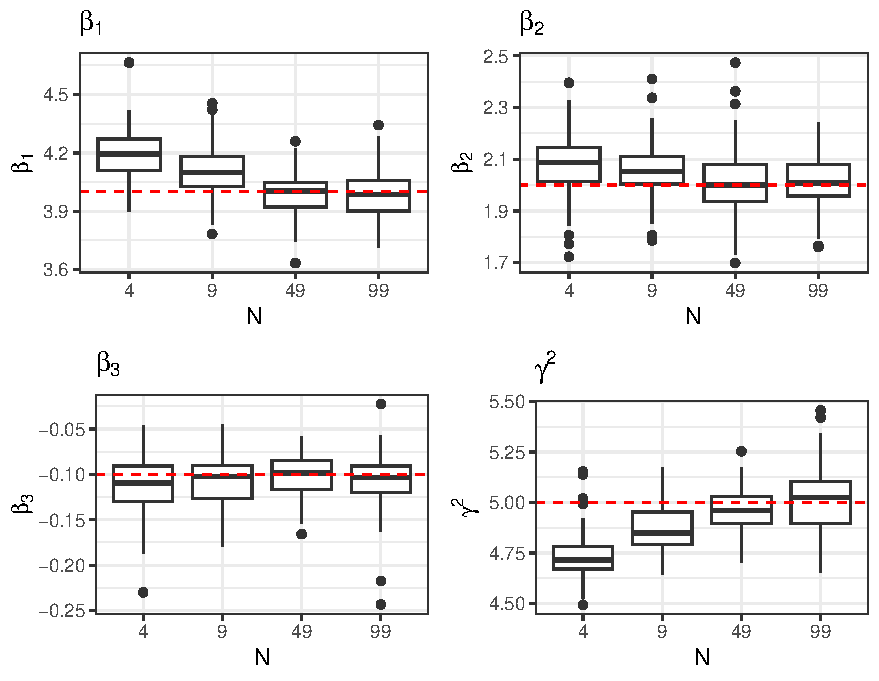
\includegraphics[width=\linewidth]{Images/Results/varying N estimates BB.pdf}
    \caption[Box plots of Parameter Estimates using Brownian bridge importance sampling using different number of bridge nodes]{box plots showing how the parameter estimates using the importance sampling estimator is affected by how many nodes N are used in the Brownian bridges. The red dotted lines show the true values of the parameters.}
    \label{fig: varying N boxplots brownian bridge}
\end{figure}

Figure~\ref{fig: varying N boxplots brownian bridge} shows that as the number of bridge nodes decreases, there is an increase in the bias of the estimates. For the $\bm \beta$-parameters, this bias is ind direction away from zero, while for $\gamma^2$ is in the direction of zero. the figure also shows that for $N=99$ and $N=49$ there is little to no bias observed in the estimates. $N = 49$ gives the same resolution for the Brownian bridges as the Langevin simulations, and $N=49$ gives half the resolution for the Brownian bridges as the Langevin simulations.

\begin{figure}[H]
    \centering
    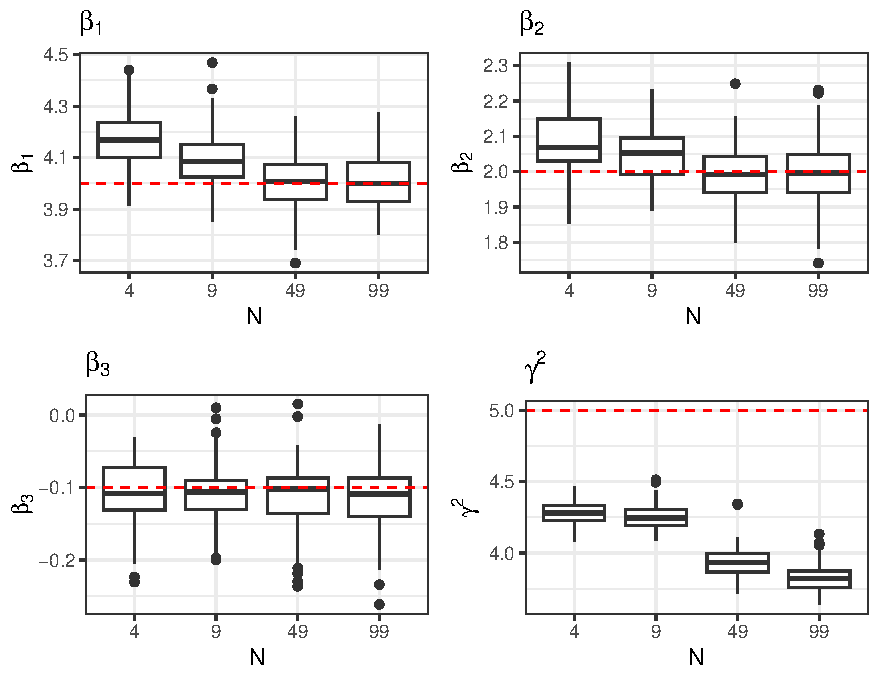
\includegraphics[width=\linewidth]{Images/Results/varying N estimates precomputed BB.pdf}
    \caption[Box plots of Parameter Estimates using pre-computed Brownian bridge importance sampling using different numbers of bridge nodes]{box plots showing how the parameter estimates using the importance sampling estimator, with pre-computed Brownian bridges is affected by how many nodes N are used in the Brownian bridges. The red dotted lines show the true values of the parameters.}
    \label{fig: varying N boxplots precomputed brownian bridge}
\end{figure}

Figure~\ref{fig: varying N boxplots precomputed brownian bridge} shows that for $N=99$ and $N=49$ there is no observable bias in the estimates of $\bm \beta$. As the number of nodes in the bridges decreases however, there is an increasing bias observed for $\beta_1$ and $\beta_2$. This bias is in the direction away from zero Which is the opposite direction of the bias we observe for the EM method when there are large distances between observations. For $\gamma^2$ there is a bias for all values of $N$ tested, which is consistent with what was experienced for this value of $\Delta_t$ in figure~\ref{fig:varying thin boxplot precomputed BB}. Unlike what was experienced with $\bm \beta$, the bias in the $\gamma$-estimates is reduced as the number of bridge-nodes decreases.

\subsection{Scenario 3}
To study the effect of the number of bridges $M$ on the estimates using the importance sampling likelihood with precomputed Brownian bridges, 100 tracks were simulated from the Langevin process, having 5000 observations and $\Delta_t = 1$. each track was estimated using the likelihood approximations with numbers of bridges $M=\{5,10,50,100,200\}$ and $N=49$ bridge nodes. The resulting estimates using the Brownian bridge importance sampling likelihood are displayed in figure~\ref{fig:varying M boxplots brownian bridge}, and the reults using pre-computed Brownian bridges are shown in figure~\ref{fig:varying M boxplots precomputed brownian bridge}


\begin{figure}[H]
    \centering
    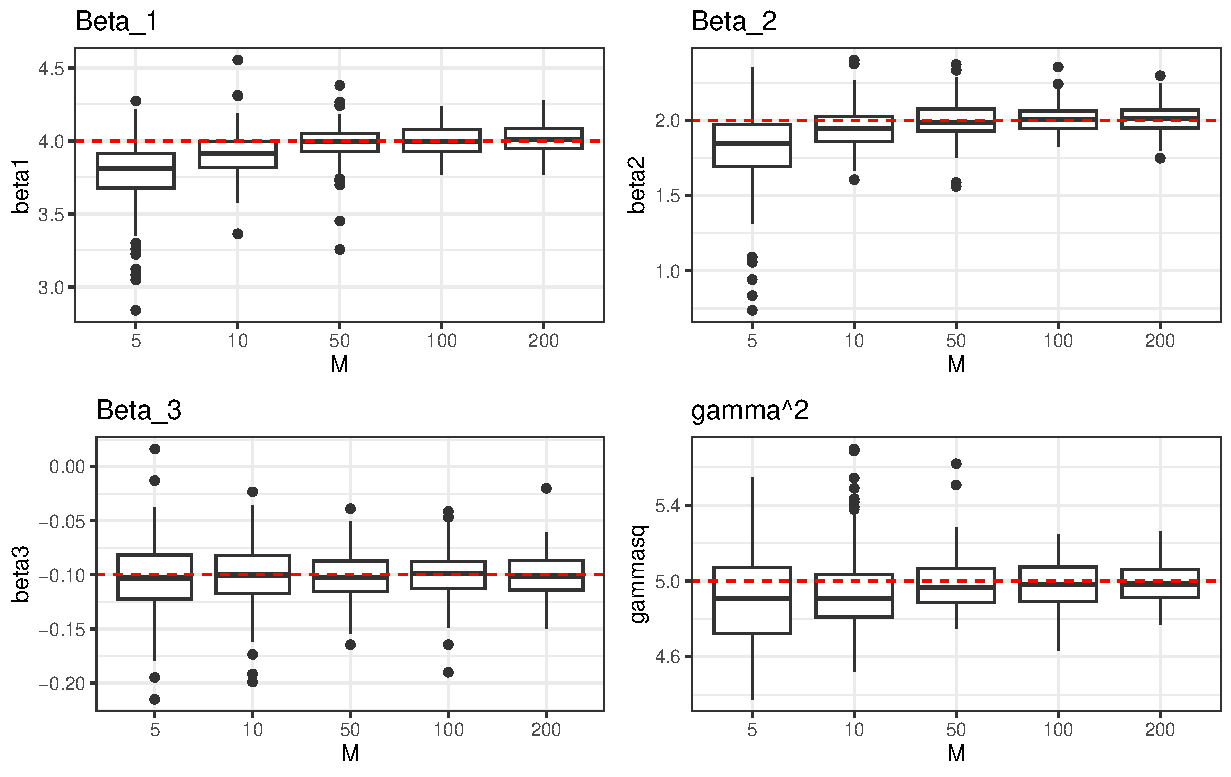
\includegraphics[width=\linewidth]{Images/Results/varying M estimates boxplot BB.pdf}
    \caption[Box plots of Parameter Estimates using Brownian bridge importance sampling using different numbers of bridges]{box plots showing how the parameter estimates using the importance sampling estimator is affected by how many bridges M are used. The red dotted lines show the true values of the parameters.}
    \label{fig:varying M boxplots brownian bridge}
\end{figure}

Figure~\ref{fig:varying M boxplots brownian bridge} shows that there are biases in the estimates of all the parameters using Brownian bridge importance sampling likelihood when the number of bridges used $M$ is small. These biases decrease as the value of $M$ increases, and for $M$ greater or equal to 100 there is no bias observed in the figure. at $M =50$ there is no bias for the $\bm \beta$ parameters but a small bias for the $\gamma^2$ estimates. Another observation is that as the variance of the estimates decreases as $M$ increases.



\begin{figure}[H]
    \centering
    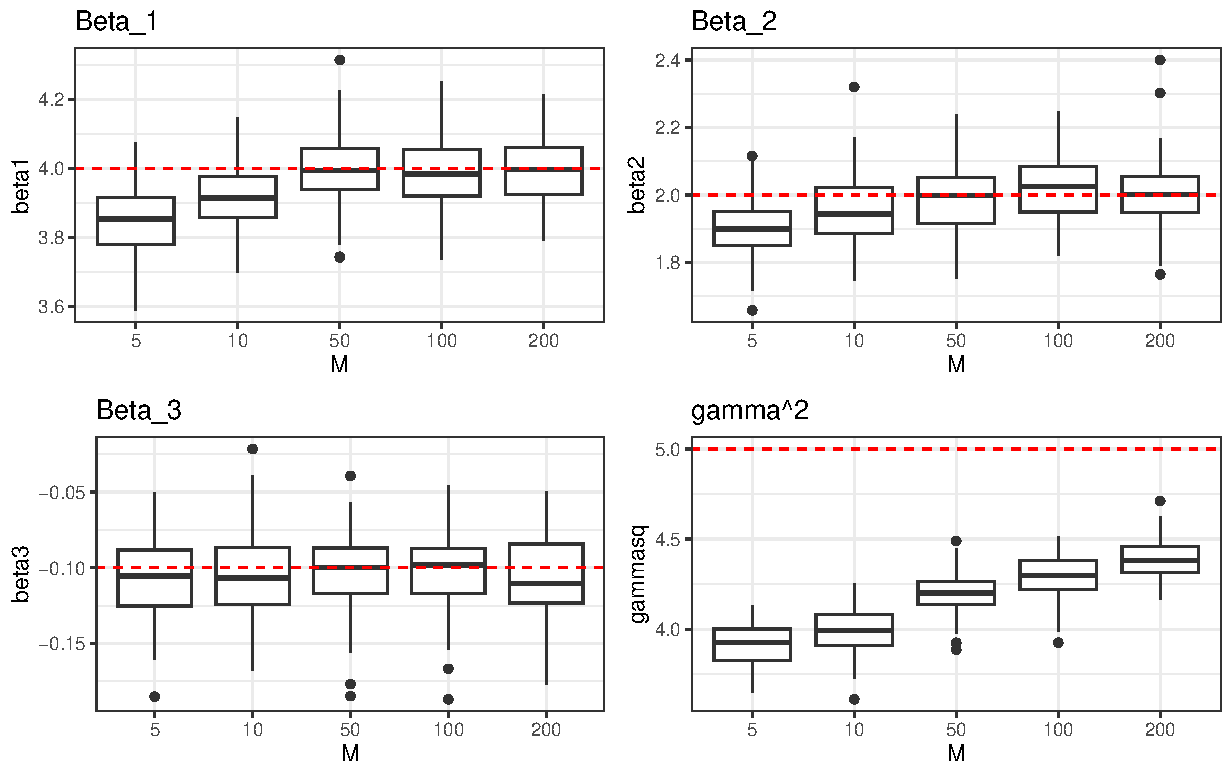
\includegraphics[width=\linewidth]{Images/Results/varying M estimates boxplot precomputed BB.pdf}
    \caption[Box plots of Parameter Estimates using pre-computed Brownian bridge importance sampling using different numbers of bridges]{box plots showing how the parameter estimates using the importance sampling estimator, with pre-computed Brownian bridges is affected by how many bridges M are used. The red dotted lines show the true values of the parameters.}
    \label{fig:varying M boxplots precomputed brownian bridge}
\end{figure}

Figure~\ref{fig:varying M boxplots precomputed brownian bridge} shows that there is a large bias in the estimate of $\gamma^2$ for all values of $M$ tested. In addition there is a bias in $\beta_1$ and $\beta_2$ when $M$ is small. The biases observed decrease as $M$ increses, and for $M$ greater or equal to 50 there is no bias observed in the estimates of $\bm \beta$. Unlike what was observed in figure~\ref{fig:varying M boxplots brownian bridge}, the variance here is stable for all values of $M$.


\subsection{Testing Computation Time}
To test the time taken to estimate the parameters of tracks using the importance sampling likelihood approximation with and without pre-computed Brownian bridges, 100 tracks were simulated from the Langevin process. Each of these tracks contained 5000 observations and had distance between observations $\Delta_t = 1$. the two methods were then timed while they were being used to estimated the tracks. the resulting times are displayed in table~\ref{tab: times} in minutes.



\begin{table}[H]
    \centering
    \begin{tabular}{c|c}
        precomputed & non-precomputed \\
        \hline
        9.261991 & 15.36517 \\
        9.702197 & 25.91244 \\
        10.473651 & 14.20421 \\
        10.410083 & 17.62082 \\
        9.427407 & 22.83060 \\
        10.391379 & 19.16781 \\
        10.436605 & 13.94819 \\
        9.431139 & 24.21317 \\
        10.084955 & 14.25600 \\
        9.397101  & 21.36654 \\
    \end{tabular}
    \caption[table of estimation times with and without pre-computation of Brownian bridges]{table of estimation times for ten tracks using the importance sampling likelihood estimates, both with and without precomputed Brownian bridges. estimation times with precomputed bridges are shown to the left and without to the right.}
    \label{tab: times}
\end{table}


From table~\ref{tab: times} we can calculate the mean of time for the method using pre-computed Brownian bridges to 9.901651 minutes and a mean time spent of 18.8885 for when the bridges were not pre-computed. The standard deviation using precomputed bridges was 0.5049866 minutes, and 4.48797 minutes when not using precomputed bridges. Overall, pre-computing the Brownian bridges gave shorter and less varied estimation times.




